% Skrivet av Nils

Primtal är förrädiskt oförutsägbara.
De dyker upp när du minst anar det och kan till synes bete sig oregelbundet.
Trots detta är de helt deterministiska i sin natur och gränsen för vad som är och inte är ett primtal är mycket tydlig.
Det är kanske just av denna anledning som primtalen, även i modern tid, är så intressanta att studera.


Hur många primtal finns det? Svaret är att det finns oändligt många.
Om vi istället frågar oss hur många primtal det finns som är mindre än en miljon, så är svaret inte lika lätt.
Till att börja med vet vi att primtal, med undantag för talet 2, aldrig är jämna.
Därför kan vi åtminstone utesluta vartannat tal upp till en miljon och säga att svaret är mindre än en halv miljon.
Hur går vi vidare härifrån?
Ett naturligt andra steg vore att föra samma resonemang för talet 3;
förutom just 3 så är primtal aldrig delbara med 3 och därmed borde vi kunna dra bort ytterligare en tredjedels miljon från svaret.
Detta är dessvärre inte riktigt sant.
Tal som både är jämna och delbara med 3 har ju uteslutits två gånger.
Det har alltså skett en dubbelräkning av alla tal som kan delas med 6,
men vi kan kompensera för detta genom att addera en sjättedels miljon till svaret.


Denna uppskattning är bättre vår tidigare. 
Vi skulle givetvis kunna fortsätta med talet 5 och på så sätt komma ännu närmre det faktiska svaret, 
men vi skulle också behöva hantera fler dubbelräkningar.
Den generella idén kallas för \textit{inklusions-exklusionsprincipen} och illustreras nedan för tre mängder med hjälp av figur \ref{pop.fig}.
\begin{figure}[H]
    \centering
    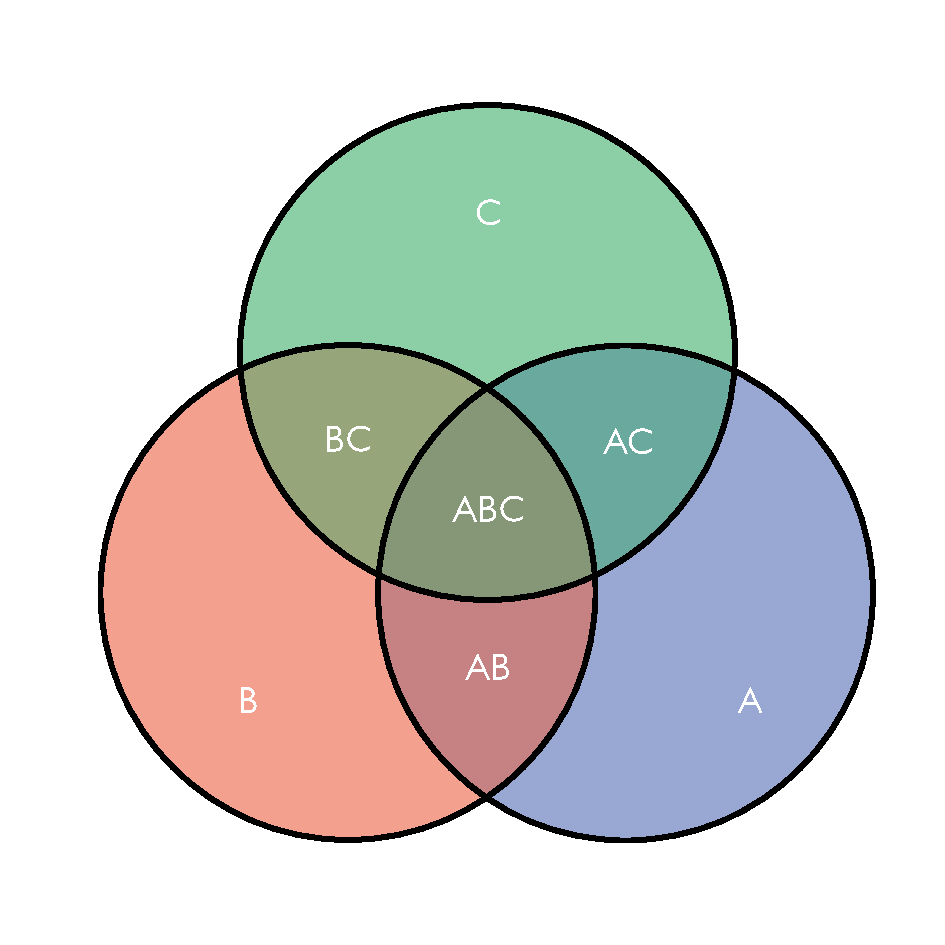
\includegraphics[scale=0.3]{erik/Images/Venndiagram.pdf}
    \caption{Illustration av inklusions-exklusionsprincipen för tre stycken överlappande mängder $A$,$B$ och $C$.}
    \label{pop.fig}
\end{figure}
Säg att vi vill uppskatta den totala storleken de överlappande mängderna $A$, $B$ och $C$. 
Vi kan börja med att summera storleken på mängderna var för sig.
Om vi betecknar storleken på $A$ som $|A|$ och gör samma sak för de andra mängderna så kan vi skriva summan som $|A|+|B|+|C|$.
Men nu har det som bekant skett en dubbelräkning av överlappen $AB$, $BC$ samt $AC$, vi drar bort dessa från summan och får $|A|+|B|+|C|-|AB|-|BC|-|AC|$.
Dessutom har vi $ABC$ där alla tre mängder överlappar varandra.
Denna ingår i alla tidigare nämnda mängder och har därmed lagts till och dragits bort tre gånger om. 
Vi lägger till $ABC$ en gång till och kommer fram till svaret
\begin{equation*}
    |A|+|B|+|C|-|AB|-|BC|-|AC|+|ABC|.
\end{equation*}
Detta är inklusions-exklusionsprincipen och den kan användas för godtyckligt många mängder.
Metoden att använda principen för att räkna primtal kallas för Legendres såll och är fundamental i teorin om matematiska såll.


Ett (matematiskt) såll är i stora drag en metod för att rensa bort vissa tal ur en större mängd.
Som ovan exempelvis, när vi använde Legendres såll för att utesluta tal som inte är primtal ur mängden av heltal upp till en miljon.
I denna rapport presenteras tre stycken såll;
Eratosthenes generaliserade såll, Bruns såll samt Selbergs såll som alla bygger på idéer liknande det vi har sett här.
Gemensamt för de tre sållen är att de inte ger något exakt svar, detta då det ofta är opraktiskt och ibland även omöjligt att erhålla ett sådant.
Istället får vi nöja oss med approximationer, vilket ändå kan vara användbart förutsatt att vi känner till storleken på felet av uppskattningen ifråga.
Det är här som de tre sållen skiljer sig åt; i sållens respektive felterm och hur denna beter sig.
Diskussion kring, och jämförelse av feltermerna är mycket relevant i sållteori och har därför tillägnas detta en egen del i rapporten.


Avslutningsvis redogör vi för hur vi, med idéer ur ett grundläggande såll kan använda datorkraft för sållning.












